%!TEX root = ../thesis.tex
%*******************************************************************************
%****************************** Third Chapter **********************************
%*******************************************************************************

\chapter{Informative targets and regularization of covariance matrix using informative targets}
\lhead{Chapter 3. \emph{New regularization method}}
\def\tr{\mbox{tr}}


% **************************** Define Graphics Path **************************

\section{Introduction} \label{sec1}
In this chapter, we use the steinian-class shrinkage estimation which is the convex linear combination of the sample covariance matix, $\boldsymbol{\hat{\Sigma}}$, and the target matrix, $\textbf{T}$, given by 
 \begin{equation}
    \hat{\boldsymbol{\Sigma}}_{\gamma}  = \gamma\textbf{T} + (1-\gamma) \hat{\boldsymbol{\Sigma}},
     \label{equ1}
     \end{equation}
where $\gamma  \in [0,1]$ is the shrinkage parameter. The target matrix need to be pre-specified and an appropriate value of $\gamma$ need to be chosen over a grid of values. Note that, when $\gamma=0$ no shrinkage is applied and the sample covariance matrix is retained, and when $\gamma=1$ full shrinkage is applied, which results $\textbf{T}$ as an estimator of the covariance matrix. \cite{ledoit2003improved} and \cite{ledoit2004well} uses identity matrix as a target estimator and the R package "corpcor" specify identity matrix as a target \citep{schaefer2013corpcor}. But sometimes it may not be a good choice as explained by \cite{schafer2005shrinkage}, the identity matrix shrinks all the diagonal and off-diagonal elements of the sample covariance matrix and consequently change the whole eigenstructure of the sample covariance matrix. \cite{schafer2005shrinkage} also discussed the six commonly used targets including identity matrix and their main focus was the diagonal matrix as a target with diagonal elements variances and off-diagonal elements zero pre-assuming that all the variables are independent, which only shrinks the eigenvalues and leave the eigenvectors intact.  

We use two more informative target matrices, that are, first order auto-regressive AR(1) and exchangeable covariance structures for which the correlation parameter, $t \in [0,1]$, is the essential element. We maximize the likelihood function of the multivariate normal distribution to choose an appropriate value of the correlation parameter as described in the next section. Next, we calculate the appropriate value of the shrinkage parameter via maximizing the likelihood function of the multivariate normal distribution. Moreover, we also obtain the optimal shrinkage intensity for the above mentioned targets by minimizing the expected quadratic loss function.    
%We use two more informative target matrices to shrink the sample covariance matrix towards them and calculate the optimal shrinkage intensity by minimizing the expected quadratic loss function. In case of these two targets the optimal shrinkage intensity rely on the correlation parameter, we maximize the likelihood function of the multivariate normal distribution to choose an appropriate value of the correlation parameter as described in the next section. In addition, we use the identity matrix as a target and choose several values of $\gamma$ to obtain the improved estimator via maximizing the likelihood function of the multivariate normal distribution. 

% First, we use the identity matrix as a target and several fixed values of $\gamma$ to obtain the improved estimator via maximizing the likelihood function of the multivariate normal distribution. Second, we use two more informative target matrices to shrink the sample covariance matrix towards them and calculate the optimal shrinkage intensity by minimizing the expected quadratic loss function. In case of these two targets the optimal shrinkage intensity rely on the correlation parameter, we maximize the likelihood function of the multivariate normal distribution to choose an appropriate value of the correlation parameter as described in the next section. 

\section{Estimation of Correlation parameter}

Correlation parameter is the essential element of the two covariance structures, namely AR(1) and exchangeable covariance structures which needs to be estimated. The AR(1) covariance structure can be defined as the first order auto-regressive structure which considers the correlation systematically decreasing with increasing the distance between the time points given by
\begin{equation}
     \sigma_{ij} = t^{|i-j|} \quad     \text{for} \quad  1 \le i,j \le p,
     \label{equ2}
\end{equation}
whereas exchangeable covariance structure can be defined as the matrix with the same covariance between variables and the variances remains constant by rearranging (exchanging) the variables given by
\begin{equation}
\sigma_{ij} = 
\begin{cases}
                                   1 & \text{when $i=j$} \\
                                   t & \text{when $i \neq j$} 
  \end{cases} \quad     \text{for} \quad  1 \le i,j \le p,
  \label{equ3}
\end{equation}
where $t$ is the constant correlation parameter and can be obtained by simply maximizing the $\log$-likelihood function of the multivariate normal distribution for both covariance structures. Let's denote the AR(1) and exchangeable covariance structures by  $\boldsymbol{\Sigma_{t}}$, the $\log$-likelihood function can be written as

 \begin{equation}
 \log L(\boldsymbol{X};\boldsymbol{\Sigma_{t}})= Const - \frac{n}{2} \log\left|\boldsymbol{\Sigma_{t}}\right|-\frac{1}{2}\boldsymbol{X^t \Sigma_{t}^{-1} X}.
 \label{equ4}
 \end{equation}
Differentiating equation \ref{equ4} with respect to $t$ we get
 \begin{equation}
 \frac{\partial}{\partial t} \log L(\boldsymbol{X};\boldsymbol{\Sigma_{t}}) = - \frac{n}{2} \frac{\partial}{\partial t} \log\left|\boldsymbol{\Sigma_{t}}\right|-\frac{1}{2} \tr \big ( \boldsymbol{X^t \frac{\partial}{\partial t} \Sigma_{t}^{-1} X} \big ).
  \label{equ5}
 \end{equation}
  Solving equation \ref{equ5} for AR(1) covariance structure the determinant of $\boldsymbol{\Sigma_{t}}$ is $\boldsymbol{|\Sigma_{t}|} = (1- t^2)^{p-1} $ and the derivative of $\log\left|\boldsymbol{\Sigma_{t}}\right|$ with respect to $t$ gives
  \begin{equation}
  \frac{\partial}{\partial t} \log |\Sigma_{t}|= \frac{-2(p-1)t(1-t^2)^{p-2}}{(1-t^2)^{p-1}}.
  \label{equ6}
  \end{equation}
The inverse of $\boldsymbol{\Sigma_{t}}$ is given by
\begin{equation*}
\Sigma_{t}^{-1}= \frac{1}{(1-t^2)}
  \begin{pmatrix}
    1 & -t & 0 & ... & 0 & 0 \\
    -t & 1+t^2 & -t & ... & 0 & 0 \\
    0 & -t & 1+t^2 & ... & 0 & 0 \\
    \vdots   & \vdots & \vdots &  \vdots &   \vdots & \vdots\\
    0 & 0 & 0 & ... & 1+t^2 & -t  \\
    0 & 0 & 0 & ... & -t & 1 \\
  \end{pmatrix}.
\end{equation*}
The derivative of $ \boldsymbol{\Sigma_{t}^{-1}}$ with respect to $t$ is given by
   \begin{equation*}
\frac{\partial}{\partial t} \Sigma_{t}^{-1}= \frac{1}{(1-t^2)^2}
  \begin{pmatrix}
    2t & -(1+t^2) & 0 & \hdots & 0 & 0 \\
    -(1+t^2) & 4t & -(1+t^2) & \hdots & 0 & 0 \\
    \vdots & \vdots & \vdots & \vdots & \vdots & \vdots \\
    0 & 0 & 0 & \hdots & 4t & -(1+t^2)  \\
    0 & 0 & 0 & \hdots & -(1+t^2) & 2t \\
  \end{pmatrix}.  
  \end{equation*}
To find $\tr \big( X^t \frac{\partial}{\partial t} \Sigma_{t}^{-1} X \big )$ in equation \ref{equ5}, we can write $\boldsymbol{X^t X = n \Sigma}$, where $\boldsymbol{\Sigma}$ is true covariance matrix with entries $\sigma_{ij}, 1 \le i,j \le p$, then
\begin{equation}
\begin{split}
n \, \tr \big ( \frac{\partial}{\partial t} \Sigma_{t}^{-1} \Sigma \big )= &\frac{1}{(1-t^2)^2} [ 2t(\sigma_{11} + 2\sigma_{22} + 2\sigma_{33} + ... + 2\sigma_{(p-1)(p-1)} + \sigma_{pp})]\\
& - t^2(\sigma_{12} + \sigma_{21} + \sigma_{23} + ... + \sigma_{(p-1)(p)} + \sigma_{p(p-1)})\\
& - (\sigma_{12} + \sigma_{21} + \sigma_{23} + ... + \sigma_{(p-1)(p)} + \sigma_{p(p-1)}),
\end{split}
\label{equ8}
\end{equation}
since $\boldsymbol{\Sigma}$ is a symmetric matrix, i.e, $\sigma_{ij}=\sigma_{ji}$ and also diagonal elements are all equal to 1, we can write equation \ref{equ8} as

\begin{equation}
n \, \tr \big ( \frac{\partial}{\partial t} \Sigma_{t}^{-1} \Sigma \big ) =\frac{2}{(1+t^2)^2} [t(p-1) - (t^2 + 1) \sum_{i=2}^{p} \sigma_{(i-1)i}].
\label{equ9}
\end{equation}
Substituting equation $\frac{\partial}{\partial t} \log |\Sigma_{t}|$ and $n \, \tr \big ( \frac{\partial}{\partial t} \Sigma_{t}^{-1} \Sigma \big )$ in equation \ref{equ5} and equating it to zero leads to
%\begin{equation*}
%\begin{split}
%\frac{\partial  L(\boldsymbol{X};\boldsymbol{\Sigma(t)})}{\partial t} =& \frac{2n(p-1)t(1-t^2)^{p-2}}{(1-t^2)^{p-1}} - \frac{2n}{2(1-t^2)^2} \big ( t(p-1)\\
%& - (t^2 + 1) \sum_{i=2}^{p} \sigma_{(i-1)i} \big ) =0,
%\end{split}
%\label{equ10}
%\end{equation*}
 \begin{equation}
 t = \frac{\sum_{i=2}^{p} \sigma_{(i-1)i}}{p-1}.
 \label{equ11}
 \end{equation}
 
If $\boldsymbol{\Sigma_{t}}$ is the exchangeable covariance structure then $|\Sigma_{t}| = (1-t)^{p-1} \lbrace 1+(p-1)t \rbrace$, differentiating $\log |\Sigma_{t}|$ with respect to $t$ gives
 \begin{equation}
    \frac{\partial}{\partial t} \log|\Sigma_{t}| = \frac{(1-t)^{p-1} (p-1) + \lbrace 1+(p-1)t \rbrace (p-1)(1-t)^{p-2}}{(1-t)^{p-1} \lbrace 1+(p-1)t \rbrace},
    \label{equ12}
   \end{equation}
 % \begin{equation}
 %log L(\boldsymbol{X};\boldsymbol{\Sigma_{ex}})= Const - \frac{n}{2} log\left|\boldsymbol{\Sigma_{ex}}\right|-\frac{1}{2}\boldsymbol{X^t \Sigma_{ex}^{-1} X}.
 %\label{equ29}
 %\end{equation}
 %Differentiating equation \ref{equ29} with respect to $t$, gives 
 %\begin{equation}
 %\frac{\partial  L(\boldsymbol{X};\boldsymbol{\Sigma_{ex}})}{\partial t} = - \frac{n}{2} \frac{\partial}{\partial t} log\left|\boldsymbol{\Sigma_{ex}}\right|-\frac{1}{2} tr \big ( \boldsymbol{X^t \frac{\partial}{\partial t} \Sigma_{ex}^{-1} X} \big ) =0,
 %\label{equ30}
 %\end{equation}
in this case the inverse of $\Sigma_{t}$ is
 \begin{equation*}
 \begin{split}
 \Sigma_{t}^{-1}=& \frac{1}{(1-t) \lbrace 1+(p-1)t \rbrace}
  \begin{pmatrix}
    1+t & -t & \hdots & -t  \\
    -t & 1+t & \hdots & -t  \\
    \vdots & \vdots & \vdots & \vdots \\
    -t & -t  & \hdots & 1+t
  \end{pmatrix}\\
&=\frac{1}{(1-t)} \big [\textbf{I} - \frac{t}{ \lbrace 1+(p-1)t \rbrace} \textbf{J} \big ],
  \end{split}
 \end{equation*}
 %\begin{equation}
  %=\frac{1}{(1-t)} \big [\textbf{I} - \frac{t}{(1+(p-1)t)} \textbf{J} \big ],
 %\label{equ13} 
 %\end{equation}
where $\textbf{I}$ is the identity matrix and $\textbf{J}$ is the unit matrix, differentiating $\Sigma_{t}^{-1}$ with respect to $t$ gives 
\begin{equation}
\frac{\partial}{\partial t} \Sigma_{t}^{-1} = \frac{1}{(1-t)^2} \textbf{I} - \Big [ \frac{1}{ \lbrace 1+(p-1)t \rbrace^2 (1-t)} + \frac{t}{\lbrace 1+(p-1)t \rbrace(1-t)^2} \Big ] \textbf{J}.
\label{equ14}
\end{equation}
The 
\begin{equation}
\begin{split}
\tr(\frac{\partial}{\partial t} \Sigma_{t}^{-1} \Sigma) =& \frac{p}{(1-t)^2} - p \big [ \frac{1}{\lbrace1+(p-1)t\rbrace^2 (1-t)} + \frac{t}{\lbrace1+(p-1)t\rbrace(1-t)^2} \big ]\\
& - \big [ \frac{1}{\lbrace1+(p-1)t\rbrace^2 (1-t)} + \frac{t}{\lbrace1+(p-1)t\rbrace(1-t)^2} \big ] \sum_{i \neq j}^{p} \sigma_{ij}.
 \end{split}   
  \label{equ15}
\end{equation}
Substituting the values of $n \, \tr(\frac{\partial}{\partial t} \Sigma_{t}^{-1} \Sigma)$ and $\frac{\partial}{\partial t} \log|\Sigma_{t}|$ in equation \ref{equ5} and equating it to zero leads to
\begin{equation}
t = \frac{\sum_{i \neq j}^{p} \sigma_{ij}}{p(p-1)}.
\label{equ16}
\end{equation}
 

\section{Estimation of regularization parameter using normal likelihood} \label{sec3}
To obtain the regularized estimator of the true covariance matrix, we propose to maximize the multivariate normal likelihood function. Given a random sample of size $n$ from $p$-variate normal distribution with mean vector, $\boldsymbol{\mu=0}$, and covariance matrix, $\boldsymbol{\Sigma}$. The log-likelihood function is
\begin{equation}
\log L(\boldsymbol{X};\boldsymbol{\Sigma})= Const - \frac{n}{2} \log\left|\boldsymbol{\Sigma}\right|-\frac{1}{2}\boldsymbol{X^t \Sigma^{-1} X}. 
\label{equ17} 
\end{equation}
In high-dimensional applications the sample estimator of the covariance matrix is not invertible, we use
\begin{equation}
\boldsymbol{\hat{\Sigma}}_{\kappa} = \boldsymbol{\hat{\Sigma}} + \kappa \boldsymbol{T},
\label{equshr}
\end{equation} 
where $\boldsymbol{T}$ is a positive definite informative target matrix and $\kappa > 0$ is the regularization parameter. The expression in \ref{equshr} incorporates additional information that we may have about the structure of the covariance matrix. If the sample size is very small, $\boldsymbol{\hat{\Sigma}}_{\kappa}$ becomes similar (if not equal) to $\boldsymbol{T}$ that is  
\begin{equation*}
\boldsymbol{T} \approx \boldsymbol{\hat{\Sigma}} + \kappa \boldsymbol{T}.
\end{equation*}
This leads to 
\begin{equation}
\kappa\boldsymbol{T} \approx \boldsymbol{T}-\boldsymbol{\hat{\Sigma}},
\label{equnshr}
\end{equation}
which can be exploited to find the value of $\kappa$ as we do later in this section.

The expression in \ref{equnshr} can also be obtained by assuming that some scaled version of $\boldsymbol{T}$ is the true covariance and replace $\boldsymbol{\Sigma}$ by $(1+\kappa)\boldsymbol{T}$ in equation \ref{equ17}, which then becomes
\begin{equation}
 \log L(\boldsymbol{X};\boldsymbol{\Sigma}_{\kappa}) = Const - \frac{n}{2} \log\left|\boldsymbol{T} + \kappa \boldsymbol{T} \right|-\frac{1}{2}\boldsymbol{X^t \frac{1}{1+\kappa}\boldsymbol{T}^{-1} X}.
 \label{equlik}
\end{equation} 
Differentiating \ref{equlik} with respect to $\kappa$ we get
\begin{equation}
\frac{\partial}{\partial \kappa} \log L(\boldsymbol{X};\boldsymbol{\Sigma}_{\kappa}) = - \frac{n}{2} (\boldsymbol{T} + \kappa \boldsymbol{T})^{-1} \boldsymbol{T} + \frac{1}{2} (\boldsymbol{T} + \kappa \boldsymbol{T})^{-1} X^t  X (\boldsymbol{T} + \kappa \boldsymbol{T})^{-1},
\label{equ18}
\end{equation}
where $\frac{\partial}{\partial \boldsymbol{\kappa}} \log |\boldsymbol{A}| = \frac{1}{|\boldsymbol{A}|} |\boldsymbol{A}| \boldsymbol{A}^{-t}$ and $\frac{\partial}{\partial \boldsymbol{\kappa}} \boldsymbol{A}^{-1} = -\boldsymbol{A}^{-1} \frac{\partial A}{\partial \boldsymbol{\kappa}} \boldsymbol{A}^{-1}$. Equating equation \ref{equ18} to zero leads to
\begin{equation*}
 \kappa \boldsymbol{T} = \boldsymbol{S} - \boldsymbol{T},
\end{equation*}
which is similar to the expression in \ref{equnshr} up to a sign which does not make difference when we ignore the sign (take the absolute) as we do in what follows.
Taking $\norm{.}_{1}$ on both sides which is the sum of the absolute of all entries of the matrix, we have
\begin{equation}
 \norm{\kappa \boldsymbol{T}}_{1} = \norm{\boldsymbol{S} - \boldsymbol{T}}_{1},
\label{equ19}
\end{equation}
If target $\boldsymbol{T}$ is the identity matrix then the value of $\kappa$ becomes
\begin{equation}
\kappa = \frac{\norm{\boldsymbol{S} - \boldsymbol{I}}_{1}}{p},
\end{equation}
for AR(1) covariance structure as a target $\kappa$ is
\begin{equation}
\kappa = \frac{\norm{\boldsymbol{S} - \boldsymbol{T}}_{1}}{p + 2\sum_{k=0}^{p-1} kt^{p-k}},
\end{equation}
furthermore, if target $\boldsymbol{T}$ is the exchangeable covariance structure then
\begin{equation}
\kappa = \frac{\norm{\boldsymbol{S} - \boldsymbol{T}}_{1}}{p + p(p-1)t}.
\end{equation}

In order to restrict the range of the regularization parameter between zero and one, it is more appropriate to use the correlation scale rather than the covariance scale in equation \ref{equ19}. The correlation matrix can be obtained as 
\begin{equation*}
\boldsymbol{\hat{R}} = \boldsymbol{\hat{\Sigma}_{d}^{-\frac{1}{2}}} \boldsymbol{\hat{\Sigma}} \boldsymbol{\hat{\Sigma}_{d}^{-\frac{1}{2}}},
\end{equation*}
where $\boldsymbol{\hat{\Sigma}_{d}}$ is the diagonal matrix with corresponding diagonal elements of  $\boldsymbol{\hat{\Sigma}}$. To get the regularization parameter at correlation scale we follow \cite{warton2008penalized} who rather regularized the correlation matrix (not the covariance matrix) and rescale $\kappa$ as
 \begin{equation}
 \gamma = \frac{1}{1+\kappa},
 \end{equation}
where $\gamma \in [0,1]$. The corresponding regularized estimator of the correlation matrix can be obtained as
\begin{equation}
\boldsymbol{R}_{\gamma} = \gamma \boldsymbol{\hat{R}}  + (1-\gamma) \boldsymbol{T}.
\end{equation}

\subsection{Sample properties of $\boldsymbol{\gamma}$}
We present some useful properties of the penalty term $\gamma$. First, for a fixed $p$ as $n$ increases $\gamma$ on the average decreases which indicates that the regularized estimator, $\boldsymbol{\Sigma}_{\gamma}$, is the consistent estimator of the true covariance matrix. In contrast, as $p$ increases the penalty term also decreases and give more weight to the target matrix. Second, for a fixed value of $p$ as we $n$ increases the variance of $\gamma$ tends to decrease.

 For making the above properties of $\gamma$ clear, we conduct a simulation study. We draw a sample of size $n= \lbrace 10,30,300 \rbrace$ from multivariate normal distribution with $p= \lbrace 10, 30, 100 \rbrace$ and mean vector, $\boldsymbol{\mu=0}$, and three types of $\boldsymbol{\Sigma}$, that is, the first order auto-regressive AR(1) covariance structure, exchangeable covariance structure and identity matrix. For both AR(1) and exchangeable covariance structures we consider $t=0.5$ and For each combination of $n$ and $p$ we simulate the data 1000 times and compute penalty parameter $\gamma$ for each combination of $n$ and $p$. Note that we use three types of targets mentioned in section \ref{sec3} in case of AR(1) and exchangeable covariance structures as a target, $\gamma$ depends on the correlation parameter $t$, which we estimate using \ref{equ11} and \ref{equ16} also note that the the penalty term changes with changing the target matrix. The aforementioned properties can be clearly seen in Figure \ref{Fig3.1}.
 


\begin{figure}[h]
\begin{center}$
\begin{array}{ll}
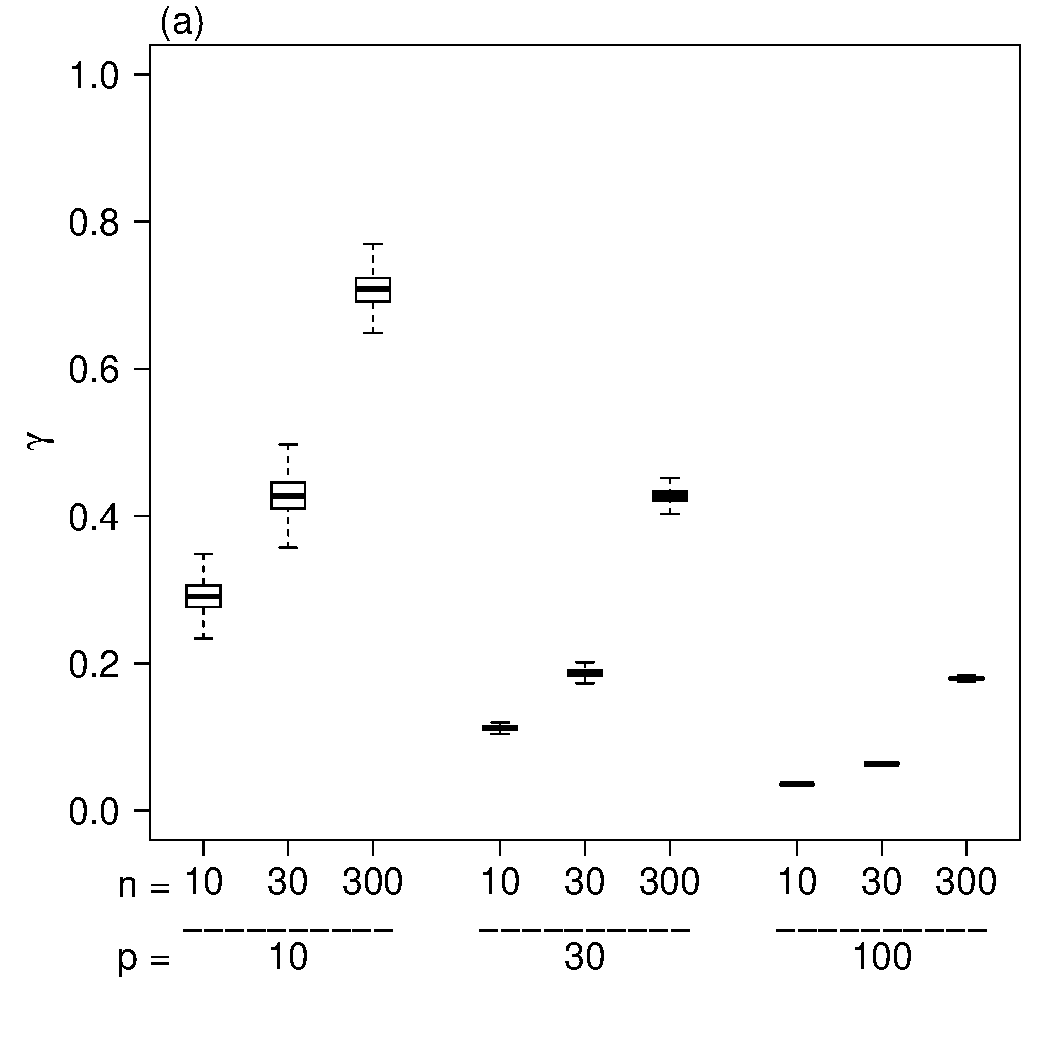
\includegraphics[scale=0.42]{boxId.pdf}
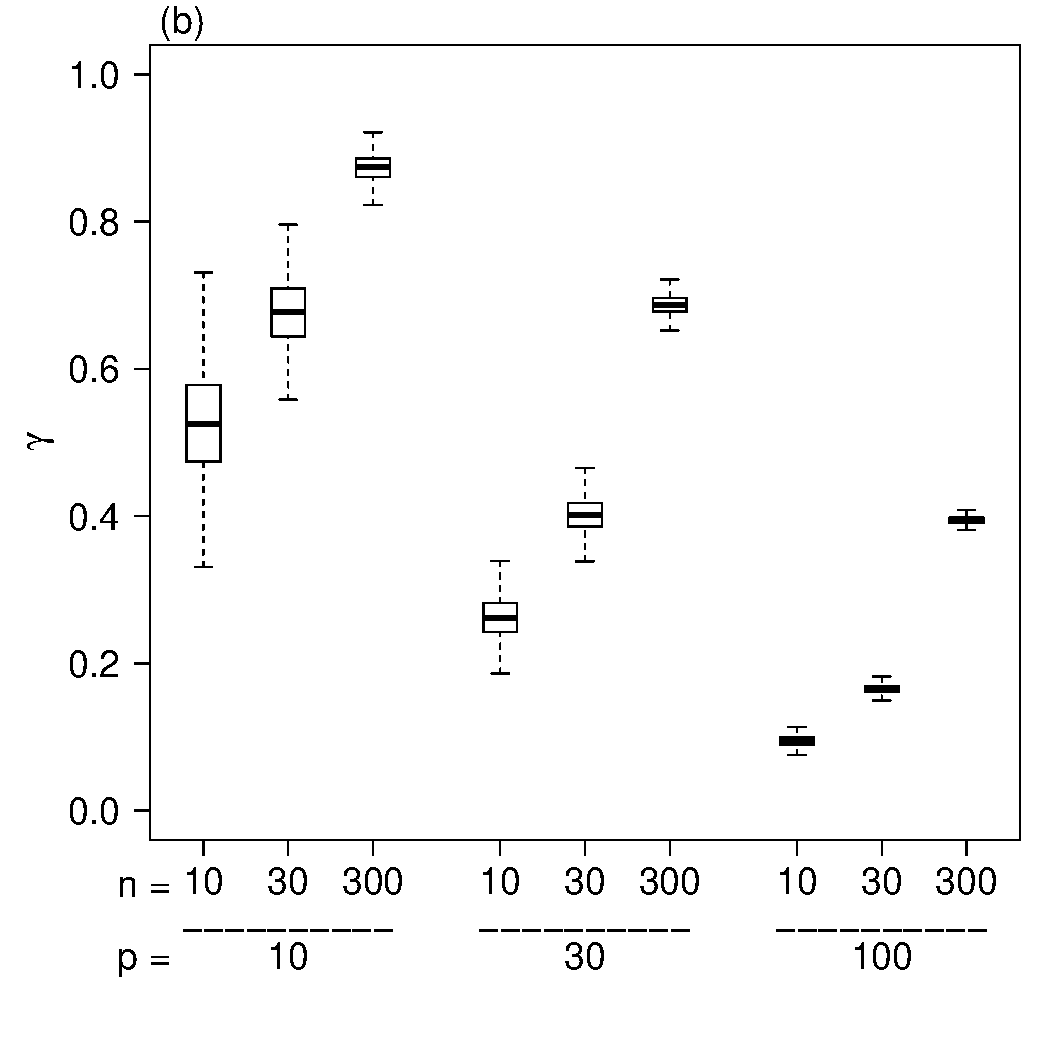
\includegraphics[scale=0.42]{boxAR.pdf}
\end{array}$
\end{center}

\begin{center}$
\begin{array}{r}
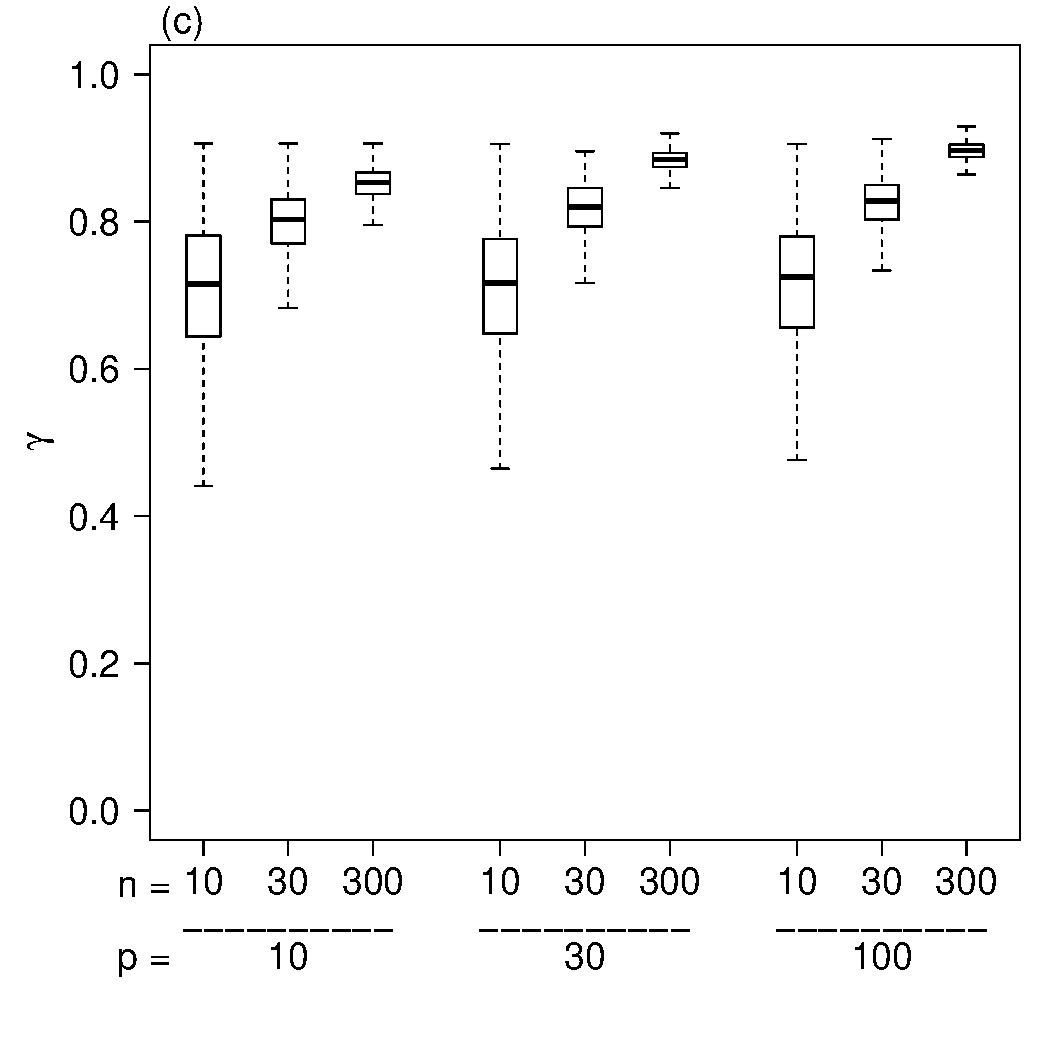
\includegraphics[scale=0.42]{boxex.pdf}
\end{array}$
\end{center}
\caption{Distribution of $\gamma$ values for different samples of size $n= \lbrace 10,30,300 \rbrace$ from a multivariate normal distribution with $p= \lbrace 10, 30, 100 \rbrace$ for different choices of $\boldsymbol{\Sigma}$ simulated 1000 times. (a) identity matrix as a true covariance matrix and as target (b) AR(1) structure as a true covariance matrix and as a target (c) exchangeable structure as a true covariance matrix and as a target.}
\label{Fig3.1}
\end{figure}